\chapter{Introduction}
%\epiquote{Websites that collect quotes are full of mistakes and never check original sources}{Randall Munroe, XKCD}
The term \emph{multimedia} describes the combination of different forms of digital media -- also called \emph{modalities} -- into a single, sensory experience that carries a higher level semantic. Those modalities include but are not limited to images and videos (visual), music, sound effects and speech (aural) or textual information. However, more exotic media types such as 3D models or signals produced by sensors can also be seen as modalities, even though experience by a human consumer may depend on pre-processing by specialized hard- and software.

Nowadays, people encounter digital media and multimedia on a daily basis when watching videos on Netflix or YouTube, when listening to music on Spotify or when browsing a private image collection on their laptop. (Multi-)media content makes up a large part of today's Internet and constitutes a major driving force behind its growth, as both volume and variety increases at an ever increasing pace. An important contributing factor are social media platforms, where users act both as consumers and producers of digital content. Current estimates suggest, that there are roughly 4.66 billion active Internet users worldwide, of which 4.2 billion can be considered active social media users\footnote{Source: Statista.com, ``Social media usage worldwide'', January 2021}. Facebook alone contributed to $144$ thousand uploaded images per minute in 2020. And many more of these  platforms, such as \emph{Instagram} or \emph{Twitter}, serve millions of users with mixed, self-made content involving text, images, videos or a combination thereof. A similar study found, that by 2025 we will produce a yearly amount of 175 Zettabytes (i.e, $10^{21}$ bytes) worth of data\footnote{Source: Statista.com, ``Big Data'', January 2021}.

Looking at these numbers, the need for efficient and effective tools for \emph{managing}, \emph{manipulating}, \emph{searching}, \emph{exploring} and \emph{analysing} multimedia data corpora becomes very apparent, which has given rise to different areas of research.

\section{Working with Multimedia Data}

On a very high level, multimedia data collections consist of individual multimedia items, such as video, image or audio files. Each item, in turn, comprises of \emph{content}, \emph{annotations} and \emph{metdata}. Unlike traditional data collections that contain only text and numbers, the content of the multimedia item itself is unstructured on a data level, which is why \emph{feature representations} that reflect a media item's content in some way and that can be handled by data processing systems are required~\cite{Zahalka:2014towards}. Traditionally, such feature representations have often been numerical vectors $f_i \in \mathbb{R}^d$. However, in theory, any mathematical object that can be processed by a computer can act as a feature. 

Multimedia analysis, which has its roots in \emph{computer vision} and \emph{pattern recognition} and started in the early 1960s and deal with the automated, computer-aided analysis of visual information found in images and later videos, i.e., the extraction and processing of feature representations. In the early days of computer vision, a lot of effort went into the engineering of feature representations that captured certain aspects of a media item's content, such as the colour distribution, texture or relevant keypoints~\cite{Lowe:1999object,Bay:2006surf} in an image. Once such features have been obtained, they can be used to perform various tasks such as classification, clustering or statistical analysis. With the advent of deep learning, the extraction of features could largely be automated through neural network architectures such as the \emph{Convolutional Neural Network (CNN)} and sometimes even be integrated with the downstream analysis~\cite{Goodfellow:2016deep}. 

Obviously, such analysis is not restricted to the visual domain and can be applied to other types of media such as speech, music, video or 3D models with specific applications, such as, speech recognition, audio fingerprinting in music, movement detection in videos or classification of 3D models, all of which fall into the broader category of multimedia analysis.

\subsection{Multimedia Retrieval}

Traditionally, multimedia retrieval or content-based retrieval could be seen as a special niche within the  multimedia analysis domain. It constitutes a dedidcated field of research that deals with searching and finding items of interest within a large (multi-)media collection. Even though this may sound like the main function of a database, it is a very different task for multimedia than it is for structured data~\cite{Blanken:2007multimedia}. On the one hand, given the structure of a relational database and languages like SQL, a user can specify exactly what elements from the database should be selected using predicates that either match or don't match the items in a collection. For example, when considering a product database that contains price information for individual items, it is trivial to formulate a query that selects all items above a specific price threshold.

Retrieving multimedia data, on the other hand, comes with indirections due to the unstructured nature of the content, the feature representations used as a proxy for it and the \emph{semantic gap} associated with these representations. A very popular model to work with the feature representations involves calculation of (dis-)similarity scores from the features and sorting and ranking of items based on this score. This is commonly referred to as the \emph{vector space model} of multimedia retrieval and similiarty search. Over the years, many different combinations of features and ranking models have been proposed to facilitate content-based retrieval of different media types, such as, images, audio or video  as have been different types of query formulation, such as \emph{Query-by-Sketch}, \emph{Query-by-Humming} or \emph{Query-by-Sculpting}~\cite{Cao:2010mind,Ghias:1995query,Boerlin:20203d}. \todo{Add sources: Survey for each modality}

Furthermore, when looking at concrete system implementations that facilitate interactive multimedia retrieval for an end-user today, the lines between multimedia retrieval and multimedia analytics quickly start to blur. This is because, in addition to the extraction of appropriate features and the conception of effective ranking algorithms, multimedia retrieval systems today also concern themselves with aspects such as query (re-)formulation and refinement, results presentation and efficient exploration~\cite{Lokovc:2019interactive}. In addition, multimedia retrieval systems do not simply operate on features representations anymore but combine \emph{similarity search} on features and \emph{Boolean retrieval} on annotations and metadata~\cite{Rossetto:2020interactive}. Therefore, one could argue that multimedia retrieval systems perform a very specific type of multimedia analytics task, which is that of finding unknown items that satisfy a specific information need. This makes all the arguments made about data processing and data management requirements for multimedia analytics applicable to multimedia retrieval as well.

\subsection{Multimedia Analytics}

Multimedia analytics aims at generating new knowledge and insights from multimedia data by combining techniques from multimedia analysis and visual analytics. While multimedia analysis deals with the different media types and how meaningful representations and models can be extracted from them, visual analytics deals with the user's interaction with the data and the models themselves~\cite{Chinchor:2010multimedia,Keim:2010mastering}. Simply put, multimedia analytics can be seens as a back and forth between multimedia (data) analysis and visual analytics, wheras analysis is used to generate models as well as visualisations from data which are then examined and refined by the user and their input. This is an iterative process that generates new knowledge and may in and by itself lead to new information being attached to the multimedia items in the collection.

\begin{figure}[h]
    \centering
    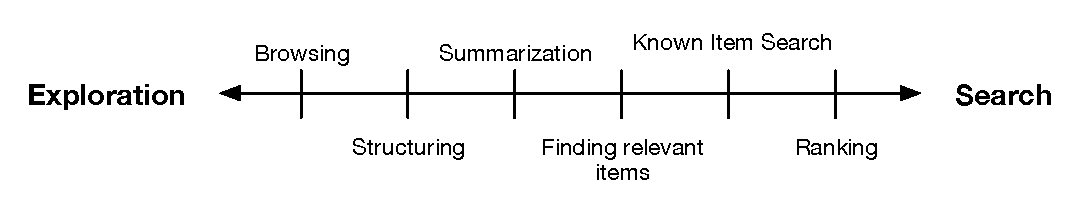
\includegraphics[width=\textwidth]{figures/exploration_search_axis.eps}
    \caption{Exploration-search axis of multimedia analytics~\cite{Zahalka:2014towards}.}
    \label{figure:exploration-search-axis}
\end{figure}

For analytics on a multimedia collection, Zahalka et al. \cite{Zahalka:2014towards} propose the formal model of an \emph{exploration-search axis}, which is depicted in \cref{figure:exploration-search-axis}. The model is used to characterize the different types of tasks carried out by the user. The axis specifies two ends of a spectrum, with \emph{exploration} marking one end -- in case the user knows nothing about the data collection -- and \emph{search} marking the other end -- in case the user knows exactly which specific items of a collection they're interested in. During multimedia analytics, a user's activities oscillate between the two ends of the spectrum until the desired knowledge has been generated. Unsurprisingly, all of the depicted activites come with distinct requirements on data transformation and processing.

As data collections become large enough for the relevant units of information -- i.e., feature representations, annotations and metadata -- to no longer fit into main memory, multimedia analytics and the associated data processing quickly becomes an issue of scalable data management~\cite{Jonson:2016}. This data management aspect becomes very challenging when considering the volume and variety of the multimedia data, the velocity at which new data is generated and the inherently unstructured nature of the media data itself.

\subsection{Dynamic Data Management}

\todo[inline]{Finetune!}

It is important to emphasize, that a media item can comprise of all of the aforementioned components and that a multimedia collection may contain items of different types. Furthermore, when looking at a media item's lifecycle, all of the aforementioned aspects are not static; annotations, metdata and features may either be generated upon the item's creation (e.g., for technical metadata), as a result of data-processing and analysis or by manually adding the information at some stage. Hence, any data management system must be able to cope with changes to that information. Those requirements are formalized in \cref{section:multmedia_data}.


\section{Research Gap and Objective}
\label{section:research_gap}

It has been pointed out by Jonson et al. \cite{Jonson:2016} (p. 296) that ``Multimedia analytics state of the art [...] has up to now [...] not explicitly considered the issue of data management, despite aiming for large-scale analytics.''. Despite recent advances and the development of concrete architecture models for multimedia database management~\cite{Giangreco:2016adam,Giangreco:2018thesis} and multimedia retrieval systems that refactor data management into distinct components~\cite{Rossetto:2018thesis}, that statement, to some extent, still holds true today. While~\cite{Giangreco:2018thesis} makes important contributions towards a unified data-, query- and execution model required for effective search and exploration in multimedia collections, scalability aspects and the need for near real-time query performance, especially in the face of dynamic data, are not systematically considered. On the contrary, the proposed models -- despite being seminal for data management in certain multimedia retrieval applications -- postulate assumptions, that have considerable impact on the practical applicability of data management systems implementing them.

The starting point for the research described in this thesis is therefore the current state-of-the-art for data management in multimedia retrieval and analytics as briefly touched upon in the previous sections. Starting from and inspired by the models and solutions proposed in \cite{Giangreco:2016adam,Giangreco:2018thesis} and motivated by the ``Ten Research Questions for Scalable Multimedia Analytics''~\cite{Jonson:2016}, this thesis challenges three basic assumptions currently employed and operated upon in multimedia data management and explores the ramifications of doing so, with the higher level goal of bridging certain gaps between research conducted in multimedia retrieval, analysis and analytics on the one hand, and classical data management and databases on the other. These assumptions are namely:

\begin{description}
    \item[Assumption 1: Staticity of data collections] Most multimedia retrieval systems today make a distinction between an \emph{offline} phase during which media items are analysed, features are generated and derived data is ingested into a data management system, and an \emph{online} phase, during which queries of the data management system take place. Usually, no changes to the data collection are being made during the online phase. This model is proposed by both \cite{Giangreco:2018thesis} and \cite{Rossetto:2018thesis} and to the best of our knowledge, most existing multimedia retrieval and analytics systems implement this either explicitly or implicitly. This simplification allows for time consuming processes related to feature extraction and indexing to take place separated from any concurrent query activities and eases requirements on transaction isolation. 

    \item[Assumption 2: Nearest neighbor search] The vector space model used in multimedia retrieval relies on a notion of similarity search that is usually expressed as finding the $k$ nearest neighboring feature vectors $\vec{v}_{i \in \left[1,k\right]} \in \mathrm{C}$ to a query vector $\vec{q} \in \mathbb{R}^d$ in a collection $\mathrm{C} \subset \mathbb{R}^d$ given a certain distance function. Very often, metrics such as the Euclidean or the Manhattan distance are employed for this comparison. While this model is very concise, computationally efficient and rather simple, it merely allows for the ranking of potential results and, given that the underlying model and the query is precise enough, finding the relevant or desired item(s).

    \item[Assumption 3: User defines execution] Database management systems usually evaluate and select the execution plan for an incoming query during a step that is refered to as \emph{query planning}. The underlying assumption here is that the database system has all the information required to determine the most effective execution path in terms of cost parameters such as required I/O, CPU and memory usage. In multimedia retrieval, this is not the case since, for example, index selection relies on a lot of different aspects that, to some extent, can be parametrized by the client issuing a query or that may be subject to change. Therefore, the index used for executing a query is often selected explicitly by the user issuing the query.
\end{description}

It is worth noting, that Assumption 1 and 3 both go against well-established design principles usually found it modern database systems.  While it may be convenient from a perspective of system design, to assume a data collection to be static, such a mode of operation is utterly limiting when considering data that is subject to change, as is the case, for example, when doing analytics or when having an application with CRUD support. A similar argument can be made for manual index selection. Such an assumption may be simplifying the process of query planning but assumes, that a user is always a technical expert. Furthermore, it limits the amount of optimization that can be applied by the data management system especially in the face of non-static data collections, where indexes are changing, or changing query workloads. 

As for Assumption 2, one can state that the described model is only able to accommodate the search-end of the \emph{exploration-search axis}, assuming that features are, in fact, real valued vectors. It quickly becomes unusable for tasks such as browsing, structuring and summarization, delegating the required data processing to upper-tier system components. Refering to \cite{Jonson:2016}, it would however be desirable to offer such primitives at the level of the data management system.

\todo[inline]{Transition from assumptions via overarching research goal to research question.}

\subsection{Research Questions}

Challenging the aforementioned assumptions raises very specific questions that fundamentaly impact the design of a \emph{multimedia data management system}. These questions are briefly summarized in \cref{table:research_questions}.

\begin{table}[h!]
    \centering
    \caption{List of research questions (RQ) resulting from challenging assumptions(AS) one, two and three.}
    \begin{tabular}{|c|p{10cm}|c|c|} 
     \hline
     \textbf{RQ} & \textbf{Question} & \textbf{Assumption} & \textbf{Domain} \\ [0.5ex] 
     \hline\hline
     1 & Which commonly used, secondary index structures for NNS (e.g., VA~\cite{Weber:1998va}, LSH~\cite{Indyk:1998lsh}, PQ~\cite{jegou:2011pq} based indexes) can cope with changes to data and to what extent? & AS 1 &\\ 
     2 & Can we estimate and quantify deterioration of retrieval quality of index structures from RQ1 as changes are being made to the underlying data collections? & AS 1 & \\ 
     3 & How can we handle index structures from RQ1 for which to expect deterioration during query planning and execution? & AS 1 & \\
     4 & Can we devise a model that (temporarily) compensates deterioration of retrieval quality of index structures? & AS 1 & \\
     5 & How can user knowledge about the the retrieval task at hand be factored into query planning without forcing the user the make explicit choices about how a query should be executed? & AS 1 \& 3 & \\
     6 & How would a cost model that factors in desired retrieval accuracy look like and can it be applied during query planning? & AS 3 & \\ 
     7 & Assuming the cost model in RQ6 exists, at what levels of the system can it be applied (globally, per query, context)? & AS 3 & \\ 
     8 & Is there a measurable impact (e.g., on query execution time vs. accuracy) of having such a cost model? & AS 3 & \\ 
     9 & Can we generalize the model for similarity search (i.e., the vector space model) and what is the consequence of doing so? & AS 2 & \\ 
     10 & Do the existing applications and use-cases justify a generalization? & AS 2 & \\ 
     \hline
    \end{tabular}
    \label{table:research_questions}
\end{table}

\todo[inline]{Associated research questions to domains (retrieval, analytics, dynamic).}

RQ1 to RQ5 address the issue of index structures for NNS, which are mostly unable to cope with data that is subject to change, since their correctness deteriorates as data is modified. The focus of these questions are whether deterioration can be quantified and how it can be handled by a system. We argue, that both is necessary for practical application in dynamic data management.

RQ6 to RQ8 explore the possibility of a cost model, that takes accuracy of the produced results into account. Since most techniques for fast NNS rely on approximation, inaccuracy is an inherent factor for such operations. Assuming such a model exists, it can be used by a user or system administrator to make explicit choices between either accuracy or execution peformance. In addition, such a cost model can be put to use when deciding what indexes to use in face of deteriorated retrieval quality due to changing data.

And finally, RQ9 and RQ10 address the issue of a more generalized model for similarity search and the impact of such a model on all the different system components. Most importantly, however, they explore and justify the need for such a model, which is not self-evident, based on concrete use-cases and applications.

\section{Contribution}

In this thesis, we try to address the research gap identified and described in \cref{section:research_gap} and thereby try to bridge the disparity between the fields of databases and retrieval systems. The contribution of this thesis can be summarized as follows:

\begin{itemize}
    \item We examine the impact of challenging the \emph{data staticity assumption} on index structures commonly used for nearest neighbor search. Most importantly, we describe a model to \emph{quantify} the effect of changing data for commonly used structures and to \emph{expose} that information to the data management system.
    \item We describe an \emph{adaptive index management} model by which a data management system can compensate errors introduced at an index level due to changes to the underlying data. The main design goal for that mechanism is, that it can be employed regardless of what type of index is used underneath.
    \item We propose a \emph{cost-model that factors-in accuracy} of generated results in addition to common performance metrics, such as IO-, CPU-, or memory-usage and, based on that model, derive mechanisms for the user to express their preference for either accuacy or speed at different levels of the system.
    \item We postulate a more \emph{generalized model for similarity search} and explore implications of such a model on aspects, such as, query planning.
    \item We introduce a working implementation that implements the aforementioned models, in the form of \emph{Cottontail DB}~\cite{Gasser:2020cottontail}.
    \item We present an evaluation of the impact of the model changes on real world datasets to provide a basis upon which their applicability can be assessed.
\end{itemize}

The described contributions are presented in four parts: The first part, to which this introduction belongs, introduces the problem and provides motivating use-cases and applications (\cref{chapter:applications}) as well as an overview of relevant research done in the fields of multimedia retrieval, multimedia analytics and data management (\cref{chapter:related_work}).

The second part, gives a brief summary of the theoretical foundation in multimedia analysis \& retrieval (\cref{chapter:theory_multimedia_analysis_and_retrieval}) and databases (\cref{chapter:theory_databases}) required to understand the remainder of this thesis. The function of these chapters is that of a refresher for readers not familiar with either domain.

The third part introduces the theoretical models that make up the aforementioned contributions (\cref{chapter:system_model}) and introduces our reference implementation Cottontail DB (\cref{chapter:cottontaildb}).

The fourth and final part presents the evaluation using Cottontail DB as an implementation (\cref{chapter:evaluation}) and discusses the conlusions and potential future work (\cref{chapter:conclusion})